\begin{frame}{Recursive Coordinate Bisection}
    
    Ranks own a subset of the elements in the mesh and the DOFs associated with those elements. 
    
    Recursive Coordinate Bisection (RCB) is used to achieve load balancing for the parallelization.

    \begin{center}
        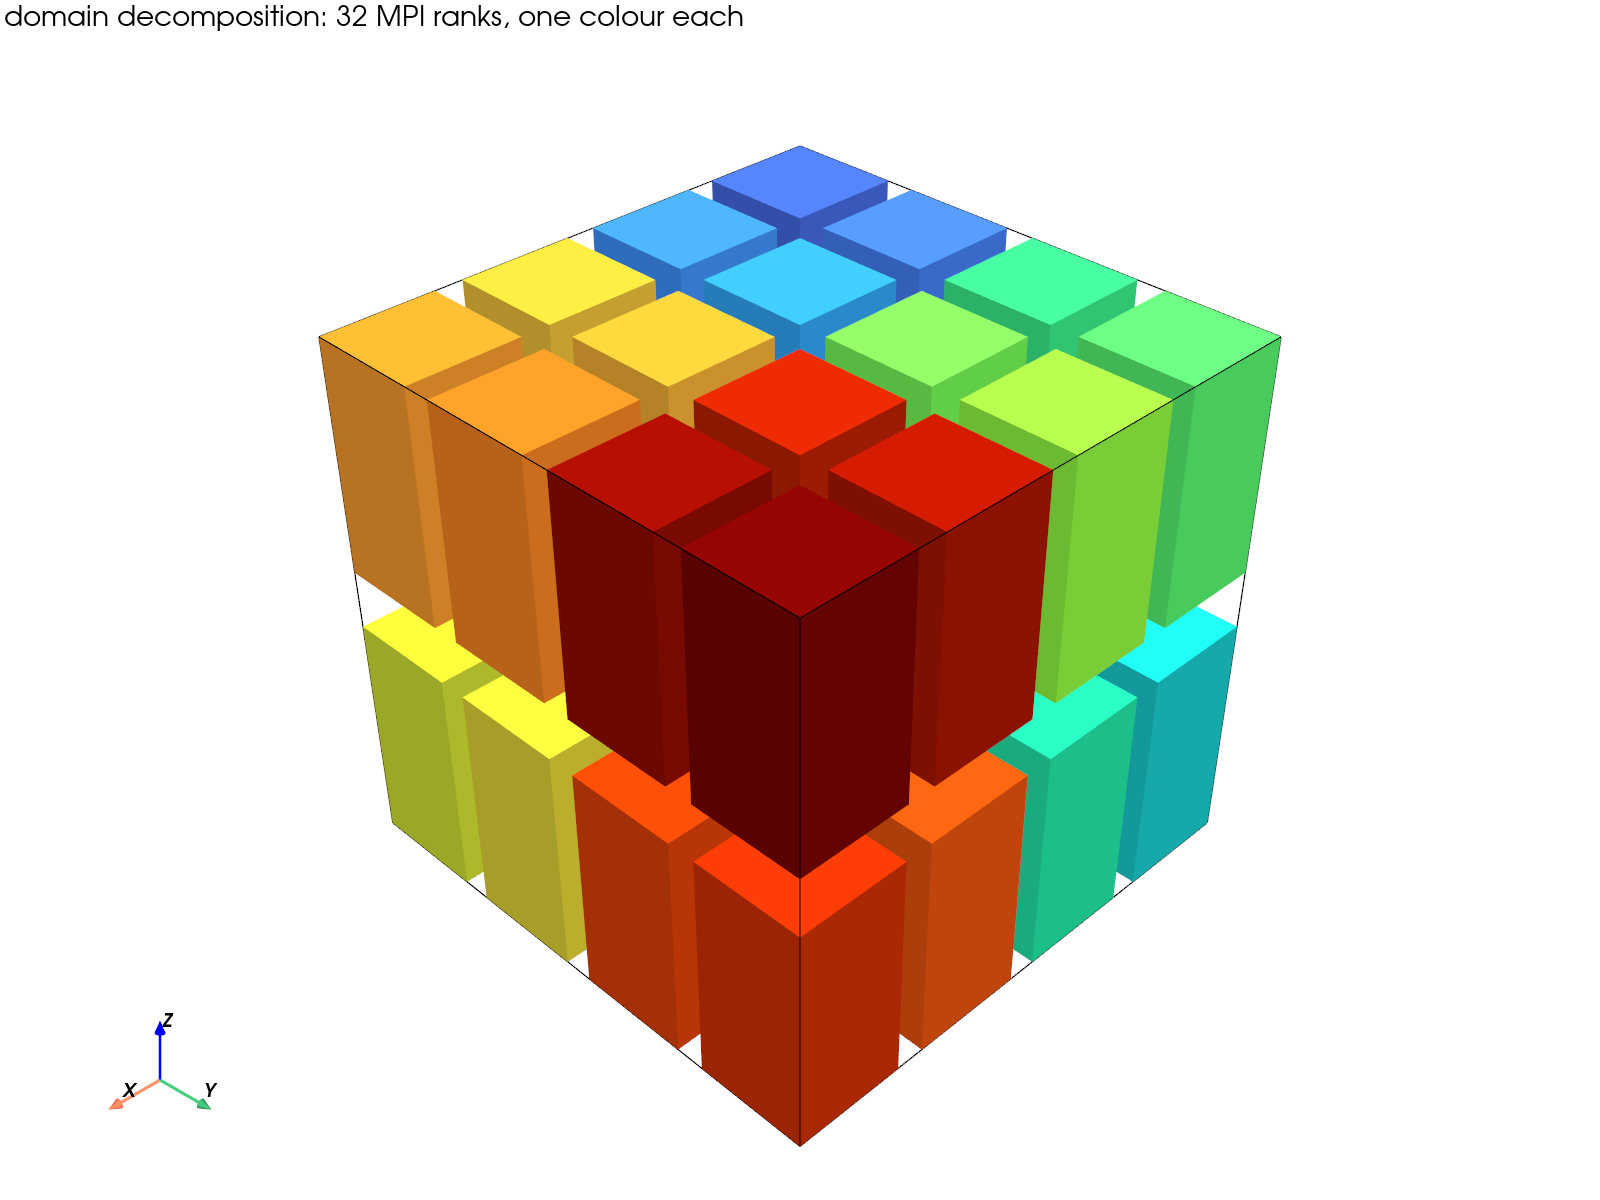
\includegraphics[width=0.49\textwidth,height=0.8\textheight,keepaspectratio]{figures/solution_ranks.png}
    \end{center}




\end{frame}

\begin{frame}{Recursive Coordinate Bisection}
    \begin{algorithm}[H]
      \caption{RCB of element set $E$ onto ranks $r_0, \dots, r_0 + P - 1$}
      \begin{algorithmic}[1]
        \Procedure{RCB}{$E$, $r_0$, $P$}
          \If{$P = 1$}
            \State assign every $e \in E$ to rank $r_0$
            \State \Return
          \EndIf
          \State $a \gets$ longest axis of the bounding box of the centroids of $E$
          \State sort $E$ by centroid coordinate along $a$ \Comment{ties: element ID}
          \State $P_L \gets \lfloor P/2 \rfloor$, \quad $P_R \gets P - P_L$
          \State $n_L \gets \lfloor \lvert E \rvert \, P_L / P \rfloor$ \Comment{elements $\propto$ ranks}
          \State \Call{RCB}{$E[1 : n_L]$, $r_0$, $P_L$}
          \State \Call{RCB}{$E[n_L + 1 : \lvert E \rvert]$, $r_0 + P_L$, $P_R$}
        \EndProcedure
      \end{algorithmic}
    \end{algorithm}
\end{frame}
